\chapter{Testování}

Testování bylo zaměřené jak na hardware, tak software. K testování docházelo postupně s rozvojem celého systému, jak dílčích částí, tak i celku. V následujícím textu jsou popsány jednotlivé softwarové části pro automatizovaný provoz a jejich výsledky při testování.

\subsection{Naměřená data pro řízení podle teplotních plánů}

Bylo provedeno měření teplotních plánů. Cílem bylo zjistit, jak dochází ke zpoždění vytápění na požadovanou teplotu vůči nastavenému časovému plánu. Měření bylo provedeno pro období od 4.~12.~2021, 00:00 do 6. 12. 2021, 21:00 pro teplotní plán místnosti „Ložnice rodičů“ (obrázek~\ref{fig:teplotni-plan-loznice-rodicu}). Teplotní úseky pro tento teplotní plán jsou od 00:00–15:00, 15:00–20:00 a 20:00–00:00.

\begin{figure}[H]
    \centering
    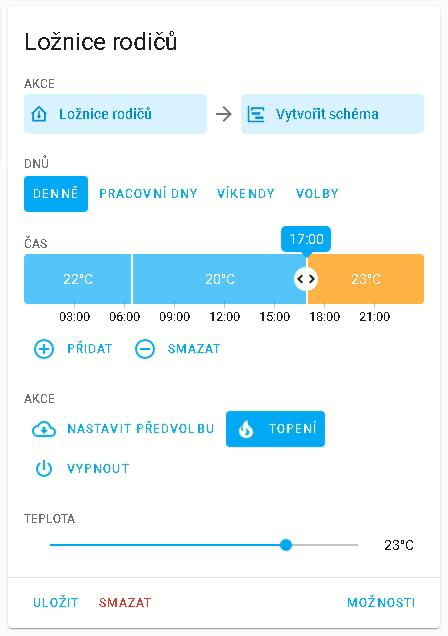
\includegraphics[width=0.4\textwidth]{images/testovani/teplotni-plany/teplotni-plan-loznice-rodicu.png}
    \caption{Teplotní plán pro místnost „Ložnice rodičů“.}
    \label{fig:teplotni-plan-loznice-rodicu}
\end{figure}

Na následujících grafech je průběh pro aktuální teplotu (modrá křivka), požadovanou teplotu (fialová křivka) a stav topení (oranžová křivka). Je popisován zkoumaný úsek pro datum 4.~12.~2021. Na obrázku \ref{fig:loznice-rodicu-termostat-zacatek-vytapeni} je začátek vytápění podle teplotního plánu v intervalu od 15:00–20:00. Podle grafu je aktuální teplota 20,9 °C, cílová je 23 °C. Této požadované teploty se dosáhne přibližně v~čase 18:00 (obrázek \ref{fig:loznice-rodicu-termostat-konec-vytepeni}), zpoždění 3 hodiny vůči začátku časového úseku. Dále podle obrázku \ref{fig:loznice-rodicu-termostat-presazeni-teploty} je vidět setrvačnost podlahového vytápění, která způsobí zvýšení teploty až na 23,8 °C.

\begin{figure}[H]
    \centering
    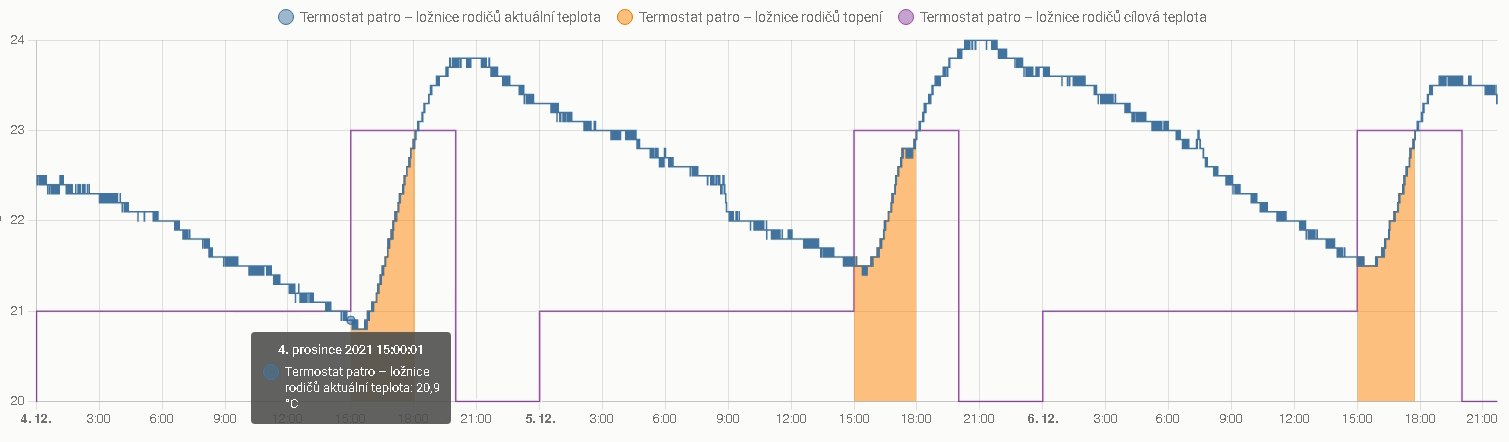
\includegraphics[width=\textwidth]{images/testovani/teplotni-plany/loznice-rodicu-termostat-zacatek-vytapeni.png}
    \caption[Naměřená data pro místnost „Ložnice rodičů“, začátek vytápění 15:00.]{Naměřená data pro místnost „Ložnice rodičů“, začátek vytápění 15:00 (zkoumaný úsek pro datum 4. 12. 2021).}
    \label{fig:loznice-rodicu-termostat-zacatek-vytapeni}
\end{figure}

\begin{figure}[H]
    \centering
    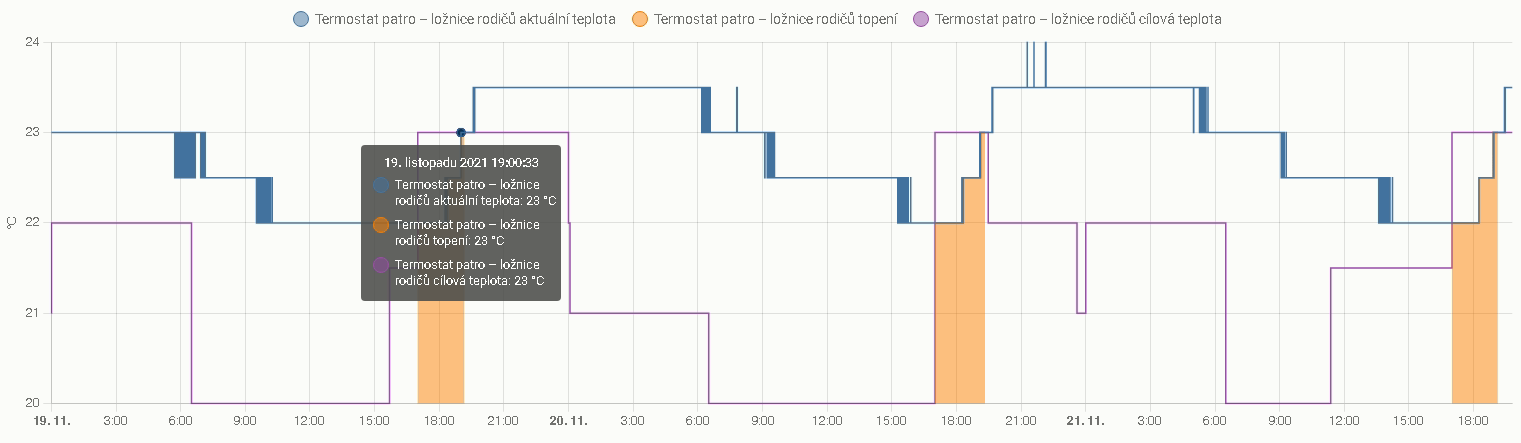
\includegraphics[width=\textwidth]{images/testovani/teplotni-plany/loznice-rodicu-termostat-konec-vytepeni.png}
    \caption[Naměřená data pro místnost „Ložnice rodičů“, dosažení požadované teploty.]{Naměřená data pro místnost „Ložnice rodičů“, dosažení požadované teploty přibližně v 18:00 (zkoumaný úsek pro datum 4. 12. 2021).}
    \label{fig:loznice-rodicu-termostat-konec-vytepeni}
\end{figure}

\begin{figure}[H]
    \centering
    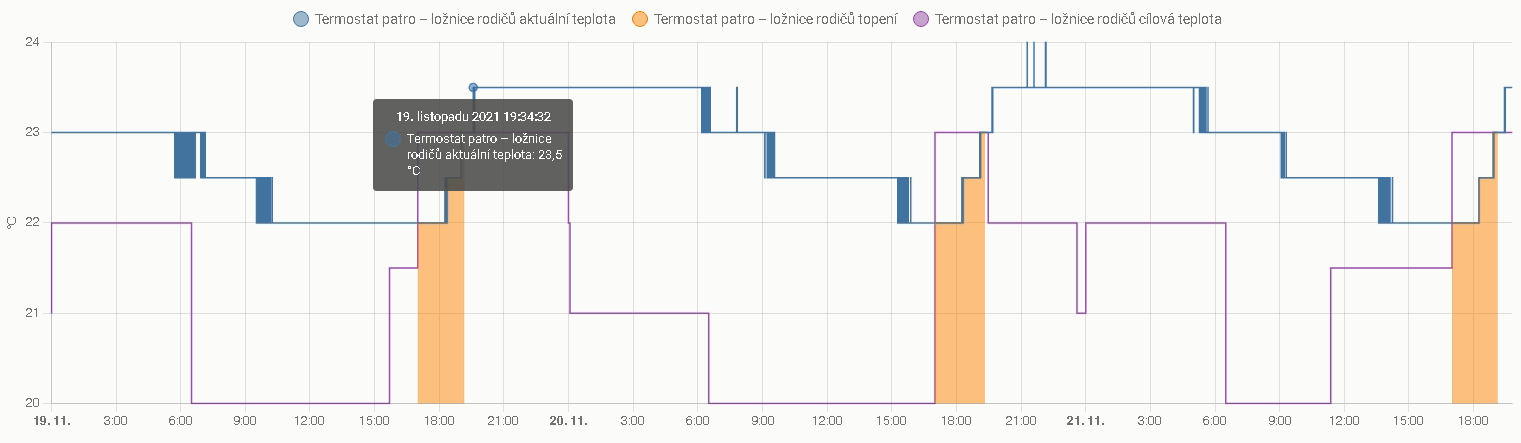
\includegraphics[width=\textwidth]{images/testovani/teplotni-plany/loznice-rodicu-termostat-presazeni-teploty.png}
    \caption[Naměřená data pro místnost „Ložnice rodičů“, přetopení místnost způsobené setrvačností podlahového vytápění.]{Naměřená data pro místnost „Ložnice rodičů“, přetopení místnost způsobené setrvačností podlahového vytápění (zkoumaný úsek pro datum 4. 12. 2021).}
    \label{fig:loznice-rodicu-termostat-presazeni-teploty}
\end{figure}

Z grafů je tedy patrné, že dojde k vytápění dané místnosti na požadovanou teplotu s~časovým zpožděním. Jednou z možností je časové plány posunout o zpoždění a dosáhnout tak v~požadovaný čas požadované tepoty, nicméně vzhledem ke změnám venkovní teploty, která má vliv na zpoždění, se nemusí dosáhnout přesně požadovaného efektu. Způsob, jak toho dosáhnout, je popsán v~textu \ref{sec:namerena-data-pro-rizeni-podle-teplotnich-planu-s-upravou-predpovedi-pocasi}. Po vypnutí vytápění místnosti dojde k jejímu přetopení v tomto případě o 0,8 °C vůči požadované teplotě 23 °C. To je způsobené setrvačností podlahového vytápění (po vypnutí ventilu je stále nahřátá voda v potrubí podlahového vytápění, dále okolní vzduch ohřívají sálající a osálané plochy v místnosti).

\subsection{Naměřená data pro řízení podle teplotních plánů s úpravou předpovědi počasí}
\label{sec:namerena-data-pro-rizeni-podle-teplotnich-planu-s-upravou-predpovedi-pocasi}
Na obrázku \ref{fig:linearni-predikce} je graf lineární predikce pro místnost „Ložnice rodičů“. Jedná se o časový posuv vytápění v minutách (D) v závislosti na rozdílu vnitřní a venkovní teploty (t). Data v grafu jsou naměřená z období 6.–12. 12. 2021 a jsou proložena přímkou. Na základě této lineární predikce se určí časový posuv pro daný časový úsek z teplotního plánu a určí se následné posunutí vytápění, aby v požadovaný čas byla dosažena požadovaná teplota. Do predikce vstupuje předpověď počasí pro začátek daného úseku z teplotního plánu. Výsledná naměřená teplota pro místnost „Ložnice rodičů“ je vidět na grafu \ref{fig:teplotni-predikce-loznice-rodicu}, průběh pro aktuální teplotu je znázorněn modrou křivkou a požadovanou teplotu znázorňuje fialová křivka. Naměřená data jsou pro období 13.–15. 12. 2021. Požadovaná teplota je tedy dosažena v požadovaný čas podle teplotního plánu. Na obrázku \ref{fig:teplotni-predikce-ventil-loznice-rodicu} jsou stavy pro termoelektrický pohon (ventil), který ovládá teplovodní smyčku pro tuto místnost. Je vidět, že k~otevření ventilu dochází přibližně o 3 hodině dříve (zelená část), než je nastavený teplotní plán na 15:00.  

\begin{figure}[H]
    \centering
    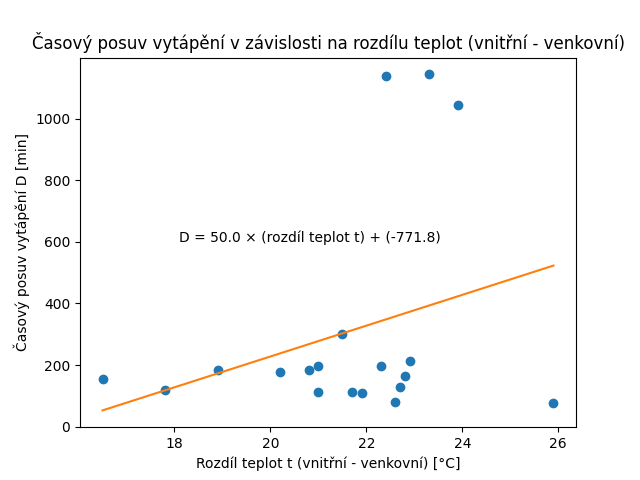
\includegraphics[width=0.8\textwidth]{images/testovani/teplotni-predikce/linearni-predikce.png}
    \caption{Lineární predikce pro místnost „Ložnice rodičů“.}
    \label{fig:linearni-predikce}
\end{figure}

\begin{figure}[H]
    \centering
    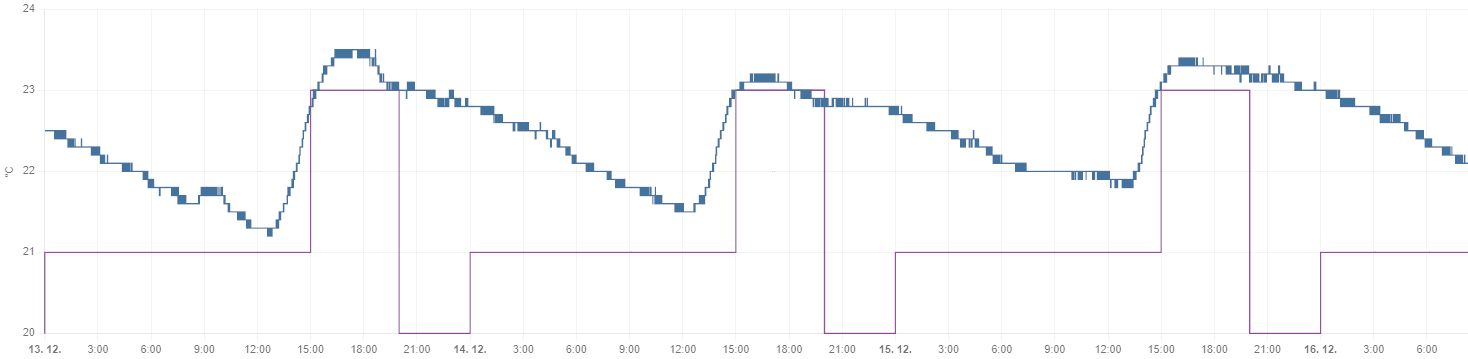
\includegraphics[width=\textwidth]{images/testovani/teplotni-predikce/teplotni-predikce-loznice-rodicu}
    \caption{Naměřená data pro místnost „Ložnice rodičů“ s teplotní predikcí.}
    \label{fig:teplotni-predikce-loznice-rodicu}
\end{figure}


\begin{figure}[H]
    \centering
    \includegraphics[width=\textwidth]{images/testovani/teplotni-predikce/teplotni-predikce-ventil-loznice-rodicu.png}
    \caption{Stavy termoelektrického pohonu (ventilu) pro místnost „Ložnice rodičů“ během teplotní predikce.}
    \label{fig:teplotni-predikce-ventil-loznice-rodicu}
\end{figure}


\subsection{Detekce otevřeného okna}
Naměřená data jsou pro místnost „Tomáš ložnice“ ze dne 18. 12. 2021 od 20:00 do 23:00. Na obrázku \ref{fig:detekce-otevreneho-okna-aktualni-pozadovana-teplota} je zobrazen pokles teploty v místnosti během otevření okna (modrá křivka) a zobrazení požadované teploty (fialová křivka). Na obrázku \ref{fig:detekce-otevreneho-okna} je zobrazení stavů pro detekci otevřeného okna. Gradient teploty pro vyhodnocení poklesu teploty je nastaven na -0,001 (změna teploty o~-0,3 °C během 5 minut). V čase 21:18 došlo k otevření okna, detekce zaznamenala otevření okna v čase přibližně 21:19. V čase 21:22 došlo k zavření okna, detekce zaznamenala zavření okna v~čase 21:32. Detekce otevřeného okna tedy funguje a její vyhodnocení bylo poměrně rychlé. Na obrázku \ref{fig:detekce-otevreneho-okna-ventil} jsou stavy pro ovládání teplovodního okruhu pro vytápění dané místnosti. Je vidět, že systém správně vyhodnotil otevřené okno a~neumožnil znovu vytápět místnost na požadovanou teplotu (23 °C), opětovné vytápění se obnovilo v čase 21:32, tedy v čase, kdy systém vyhodnotil, že okno je již zavřené. Problém nastává především u větších místností, kde trvá delší dobu, než se vyhodnotí pokles teploty (čím nižší venkovní teplota, tím rychleji vnitřní teplota klesá). Řešením může být nastavení menšího gradientu teploty pro danou místnost. Zde je však nutné správné nastavení, aby nedocházelo k detekci otevřeného okna i v případech, kdy okno je zavřené, ale dochází k~požadovanému poklesu teploty v~místnosti (v rámci teplotního plánu).

\begin{figure}[H]
    \centering
    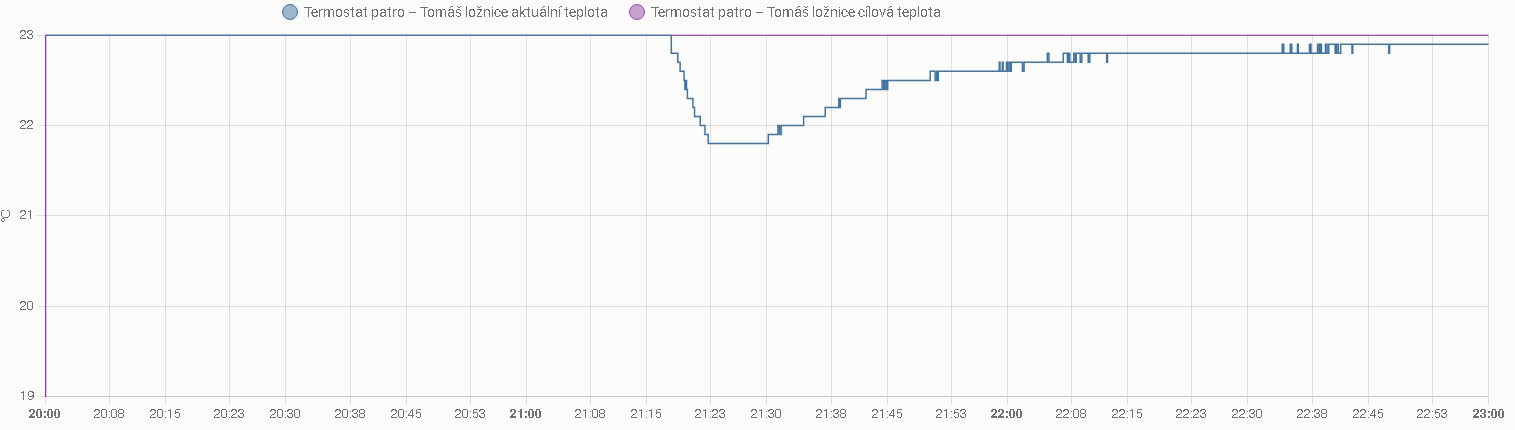
\includegraphics[width=\textwidth]{images/testovani/detekce-otevreneho-okna/detekce-otevreneho-okna-aktualni-pozadovana-teplota.png}
    \caption{Aktuální a požadovaná teplota během detekce otevřeného okna pro místnost „Tomáš ložnice“.}
    \label{fig:detekce-otevreneho-okna-aktualni-pozadovana-teplota}
\end{figure}

\begin{figure}[H]
    \centering
    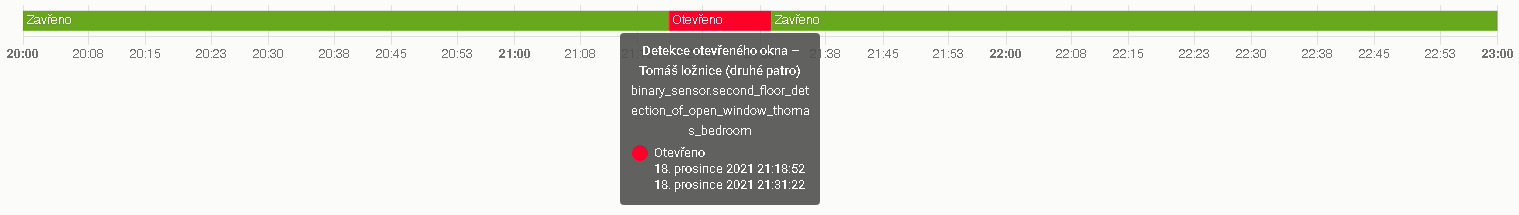
\includegraphics[width=\textwidth]{images/testovani/detekce-otevreneho-okna/detekce-otevreneho-okna.png}
    \caption{Stavy detekce otevřeného okna pro místnost „Tomáš ložnice“.}
    \label{fig:detekce-otevreneho-okna}
\end{figure}

\begin{figure}[H]
    \centering
    \includegraphics[width=\textwidth]{images/testovani/detekce-otevreneho-okna/detekce-otevreneho-okna-ventil.png}
    \caption{Stavy termoelektrického pohonu (ventilu) pro místnost „Tomáš ložnice“ během detekce otevřeného okna.}
    \label{fig:detekce-otevreneho-okna-ventil}
\end{figure}


%\begin{figure}[H]
%    \centering
%    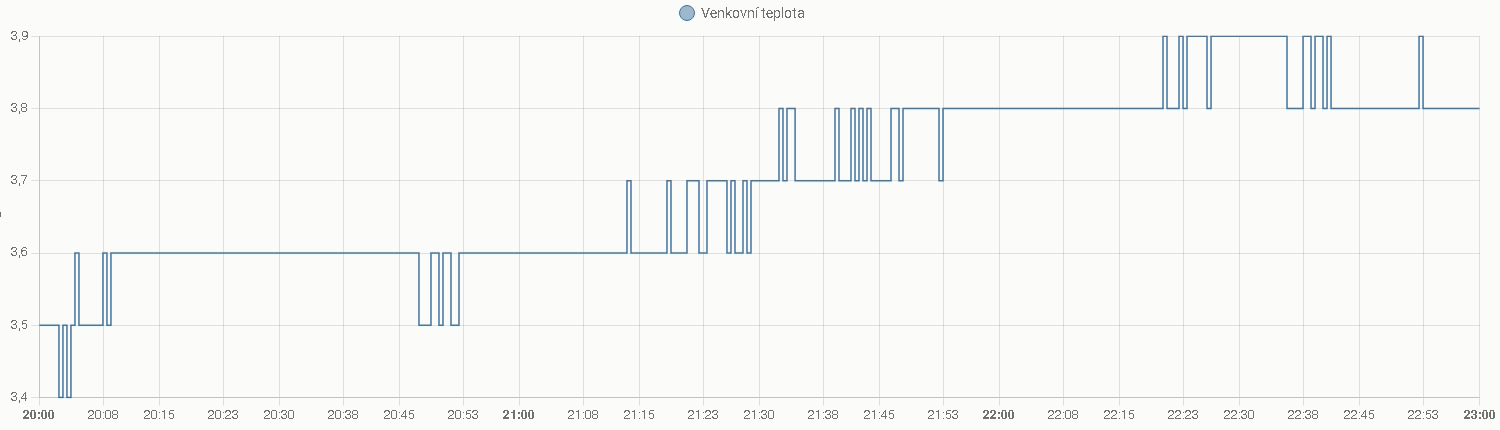
\includegraphics[width=\textwidth]{images/testovani/detekce-otevreneho-okna/detekce-otevreneho-okna-venkovni-teplota.png}
%    \caption{}
%    \label{fig:detekce-otevreneho-okna-venkovni-teplota}
%\end{figure}

